\documentclass[12pt]{article}
\usepackage[a4paper,top=3cm,bottom=3cm,left=2.5cm,right=2.5cm]{geometry}
\usepackage[italian]{babel}
\usepackage[utf8x]{inputenc}
\usepackage {caption}
\usepackage {amsmath}
\usepackage {kbordermatrix}
\usepackage {url}
\usepackage {multirow}
\usepackage {booktabs}
\usepackage {fixltx2e}
\usepackage {float}
\usepackage {graphicx}
\usepackage {cite}
\usepackage {listings}
\usepackage {color}
\usepackage {xcolor,colortbl}
\usepackage {adjustbox}
\usepackage {array}
\usepackage {svg}
\usepackage {subfig}
\usepackage {amssymb}
\usepackage {hyperref}
\usepackage {tabulary}
\usepackage {tabularx}
\usepackage[T1]{fontenc}
\usepackage{wasysym}
\usepackage{enumitem}
\usepackage{lipsum}

\usepackage{charter} %font

\usepackage[titletoc]{appendix}


\newcommand{\voceU}[1]{%
	\item #1\dotfill\Square%
}

\newcommand{\voceD}[1]{%
	\item #1\hfill\Square%
}
\hypersetup{colorlinks=true,citecolor=black,linkcolor=black, urlcolor=blue}

\date{}

\renewcommand{\lstlistingname}{Listato}


\definecolor{dkgreen}{rgb}{0,0.6,0}
\definecolor{gray}{rgb}{0.5,0.5,0.5}
\definecolor{mauve}{rgb}{0.58,0,0.82}

\lstdefinestyle{scalacode}{
	frame=tb,
	language=scala,
	aboveskip=3mm,
	belowskip=3mm,
	showstringspaces=false,
	columns=flexible,
	basicstyle={\small\ttfamily},
	numbers=none,
	numberstyle=\tiny\color{gray},
	keywordstyle=\color{blue},
	commentstyle=\color{dkgreen},
	stringstyle=\color{mauve},
	frame=single,
	breaklines=true,
	breakatwhitespace=true,
	tabsize=3,
}

\lstdefinelanguage{JavaScript}{
	keywords={typeof, new, true, false, catch, function, return, null, catch, switch, var, if, in, while, do, else, case, break},
	keywordstyle=\color{blue}\bfseries,
	ndkeywords={class, export, boolean, throw, implements, import, this, Controller, },
	ndkeywordstyle=\color{orange}\bfseries,
	identifierstyle=\color{black},
	sensitive=false,
	comment=[l]{//},
	morecomment=[s]{/*}{*/},
	commentstyle=\color{purple}\ttfamily,
	stringstyle=\color{red}\ttfamily,
	morestring=[b]',
	morestring=[b]"
}

\lstset{
	frame=tb,
	language=JavaScript,
	extendedchars=true,
	basicstyle=\footnotesize\ttfamily,
	%showstringspaces=false,
	showspaces=false,
	numbers=none,
	%numberstyle=\footnotesize,
	numbersep=9pt,
	tabsize=2,
	frame=single,
	breaklines=true,
	breakatwhitespace=true,
	tabsize=3,
}

\begin{document}
\sloppy

\title{\textbf{Definizione ed Implementazione di un Sistema di Raccomandazione Distribuito per film
		e Modellazione di Eventi Complessi}}

\author{\\\textit{Prof. Ing.} Tommaso di Noia\\\textit{Prof.ssa} Marina Mongiello\\
	\textit{Dott.} Francesco Nocera\\
	Mauro Losciale\\ 
	Pietro Tedeschi\\}

\clearpage\maketitle
\thispagestyle{empty}

\begin{center}
	
\includegraphics[scale=0.40]{images/poliba.jpg}
\end{center}

{\textbf{\center Logica e Intelligenza Artificiale\\Ingegneria del Software Avanzata\\ Laurea Magistrale in Ingegneria Informatica\\Politecnico di Bari\\A.A 2015 - 2016\\}}

\newpage
\clearpage
\thispagestyle{empty}
\renewcommand\contentsname{Indice}
\tableofcontents
\newpage
\setcounter{page}{1}

\newpage
\section{Introduzione}
La crescente diffusione dei contenuti digitali e l'incremento pervasivo dei dispositivi tecnologici I sistemi di raccomandazione sono degli strumenti che suggeriscono in modo personalizzato i prodotti utili che potrebbero interessare un utente, in base ai propri interessi. L'elenco degli elementi in output è il risultato di un processo decisionale, che ha l'obiettivo di dedurre quali sono le preferenze dell'utente ed aiutarlo a scegliere il prodotto a lui più indicato. I sistemi di raccomandazione, coinvolgono settori multidisciplinari che vanno dall'interazione uomo-macchina, all'intelligenza artificiale, dalla sicurezza informatica, al supporto decisionale. Esempi cardini di sistemi raccomandazione sono Google News per le notizie, Netflix per i film, Amazon per l'e-commerce, Last.fm per la musica.

Il tema d'anno ha lo scopo di costruire un sistema di raccomandazione distribuito, utilizzabile con un'interfaccia web, che sia in grado di analizzare lo stream dati in input, gestendo gli eventi complessi mediante query continue sul flusso informativo. Il sistema di raccomandazione consentirà di votare un numero di film che sia strettamente maggiore di tre, selezionando i contenuti votati con un rate superiore o uguale a quattro, al fine di raccomandare i film non ancora visti, che si avvicinano di più ai gusti dell'utente.
\section{Stato dell'arte}

\subsection{Introduzione ai sistemi CEP}
L'incremento dei dispositivi interconnessi e delle applicazioni distribuite, richiede un'elaborazione continua del flusso dati. Esempi di tali applicazioni, vanno dal traffico generato dalle Wireless Sensor Networks (WSN) al flusso dati relativo agli indici finanziari, dal monitoraggio stradale alla Clickstream Analysis. 

Un sistema ad eventi complessi, meglio conosciuto come \textit{Complex Event Processing} (CEP), modella il flusso informativo dei dati, visualizzando gli elementi come notifiche di ciò che sta accadendo nel mondo esterno. I dati vengono rilevati e filtrati utilizzando dei pattern (oppure le \textit{processing rules}), i quali hanno il compito di rappresentare il modello di riferimento con l'informazione da rilevare, per poi farla pervenire alle rispettive parti (ad esempio, i dispositivi che effettuano una sottoscrizione ad un determinato topic nel paradigma \textit{publish-subscribe}). L'obiettivo di un sistema CEP consiste nell'identificare eventi significanti e rispondere ad essi nel più breve tempo possibile.
Un pattern o una regola, può essere definita mediante un linguaggio basato su query, il cosiddetto \textbf{Event Query
	Language}.
\begin{figure}[H]
	\centering
	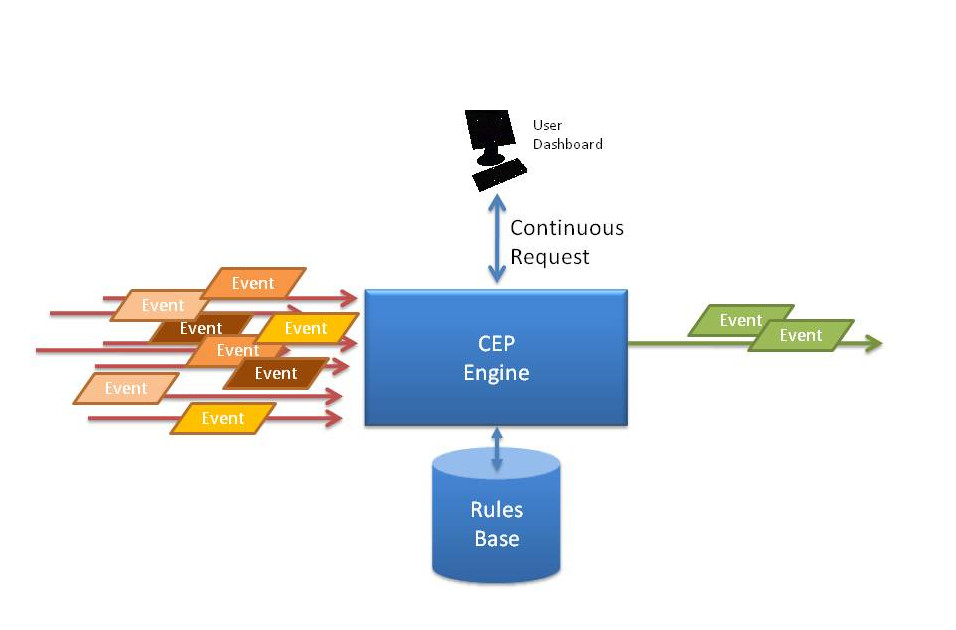
\includegraphics[scale=0.50]{images/CEP2.jpg}
	\caption{Architettura di un Sistema CEP\cite{cepimage}}
	\label{archcep}
\end{figure}

Gli \textbf{Event Query Languages} possono essere raggruppati in tre categorie: Composition Operators, Data Stream Query Languages e
Production Rules. I Composition Operators identificano gli eventi complessi partendo dalla composizione dei singoli eventi, utilizzando operatori quali congiunzione, negazione o di sequenza per la costruzione delle espressioni. Esempi rilevanti sono IBM Active Middleware Technology e ruleCore. 

I \textbf{Data Stream Query Languages} sono basati sul linguaggio SQL; gli stream di dati sono semplicemente tuple convertite per database relazionali, in modo che si possano eseguire query SQL su di esse. E' utile citare i seguenti approcci: CQL, Coral8, StreamBase,
Aleri, Esper e così via.

Le \textbf{Production Rules} specificano le azioni che devono essere eseguite quando il sistema si trova in determinati stati; non è un linguaggio ad eventi, ma costituisce un approccio importante nei sistemi CEP. Un esempio pratico è TIBCO Business Events.

Un altro fattore importante è il tempo. Sono due le parti da considerare quando si parla del tempo, il tempo della finestra ed il tempo dell'evento informativo. Il tempo della finestra mostra gli eventi che vengono esaminati in un determinato intervallo. Il tempo dell'evento invece, porta con se informazioni relative alla data, ora di rilevazione, tempo di transizione, ed intervallo di elaborazione.

I contributi relativi ai sistemi CEP, arrivano da diverse comunità, a partire da quelle che si occupano di sistemi distribuiti, automazione industriale, sistemi di controllo, monitoraggio delle reti, Internet of Things, e middleware in generale.

\begin{figure}[H]
	\centering
	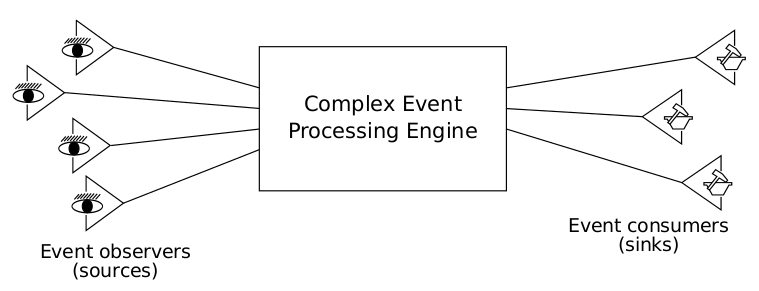
\includegraphics[scale=0.40]{images/CEP.png}
	\caption{Funzionamento di un Sistema CEP (High-Level) \cite{Cugola:2012:PFI:2187671.2187677}}
	\label{funcep}
\end{figure}

Come possiamo vedere dalla Figura \ref{funcep}, viene associata una semantica dettagliata agli elementi informativi da processare. Da una parte abbiamo gli \textbf{Event Observer}, i quali rappresentano la sorgente dei dati e degli eventi da notificare; in seguito abbiamo il \textbf{CEP Engine}, responsabile del filtraggio e della notifica degli eventi ai nodi \textit{sink}, identificati come \textbf{Event Consumers} \cite{Cugola:2012:PFI:2187671.2187677,fulop2010survey}.

\subsection{Sistemi di Raccomandazione}
I sistemi di raccomandazione, raccolgono informazioni sulle preferenze di utente in corrispondenza di un insieme di elementi (ad esempio, film, musica, libri, giochi, viaggi, siti web, applicazioni, gadget). L'informazione può essere acquisita in maniera esplicita (tipicamente ciò viene fatto acquisendo il voto di un utente) o implicitamente (analizzando il comportamento dell'utente, ad esempio musica ascoltata, applicazioni scaricate, siti web visitati, libri letti). Inoltre i sistemi di raccomandazione, possono tener conto anche delle caratteristiche demografiche dell'utente (ad esempio età, nazionalità, sesso); dei contenuti informativi presenti nel mondo del Web 2.0, ad esempio all'interno delle piattaforme di Social Networking, quali follower, followed, twit, like, post; dei dati provenienti dai dispositivi caratterizzanti l'Internet of Things (ad esempio, coordinate GPS, RFID, segnali medici inviati in real-time). 

I sistemi di raccomandazione utilizzano diverse sorgenti informative al fine di fornire all'utente finale una migliore Quality of Experience relativa alla predizione ed alla raccomandazione degli elementi che potrebbero interessargli. La tecnica del Collaborative Filtering (CF), ha un ruolo fondamentale nella raccomandazione, sebbene viene spesso usata anche con altre tecniche di filtraggio basate sul contenuto o basate sulla conoscenza. Il CF si basa sulla cronologia decisionale dell'utente: oltre alle nostre esperienze, facciamo le nostre decisioni anche in base alla conoscenza che ci circonda.

Il processo con cui un sistema di raccomandazione generi una raccomandazione, è basato sulla combinazione delle seguenti considerazioni:

\begin{enumerate}
\item La tipologia di dati disponibili nel databse (votazioni, informazioni di registrazione dell'utente, caratteristiche peculiari del contenuto informativo, relazioni sociali)
\item L'algoritmo di filtraggio usato (demografico, basato sul contenuto, collaborativo, basato sulle relazioni sociali, dipendente dal contesto e ibrido).
\item Il modello scelto (basato sull'uso diretto dei dati: 'memory-based', oppure un modello generato usando tali dati: 'model-based').
\item Le tecniche impiegate: approccio probabilistico, reti Bayesiane, algoritmi di tipo nearest neighbors, algoritmi genetici, reti neurali, logica fuzzy.
\item Livello di dispersione del database e scalabilità desiderata.
\item Capacità di elaborazione del sistema (tempo di elaborazione e consumi di memoria).
\item L'obiettivo da raggiungere (predizioni e raccomandazioni)
\item La qualità del risultato desiderata (ad esempio la precisione).
\end{enumerate}

La ricerca nell'ambito dei sistemi di raccomandazione, richiede che i dati siano di dominio pubblico, al fine di semplificare la ricerca sulle tecniche innovative relative all'analisi dei dati. Esempi di dataset pubblici presenti in letteratura, sono Last.Fm, Delicious, Netflix, MovieLens.
Le funzionalità interne per i sistemi di raccomandazione, sono caratterizzate dagli algoritmi di filtraggio. 
Gli algoritmi di filtraggio vengono classificati nel modo seguente:
\begin{itemize}
	\item Collaborative Filtering
	\item Demographic Filtering
	\item Content-Based Filtering
	\item Hybrid Filtering
\end{itemize}

Il \textbf{Content-Based Filtering} consente di creare raccomandazioni basate sulle scelte fatte in passato da un utente (ad esempio, in un sito E-Commerce, se l'utente ha acquistato una fiction cinematografica, probabilmente il sistema di raccomandazione gli consiglierà una fiction recente, che non ha ancora acquistato sul sito). La tecnica consente inoltre di generare la raccomandazione utilizzando il contenuto dell'oggetto, ad esempio il testo, le immagini, l'audio.

Il \textbf{Demographic Filtering} si basa sul principio che gli individui con caratteristiche personali comuni, quali età, sesso, luogo di residenza e così via, avranno le stesse preferenze.

Il \textbf{Collaborative Filtering} consente agli utenti di attribuire un voto ad un insieme di elementi (filmati, canzoni, film, libri, all'interno di una piattaforma web) salvando le proprie preferenze all'interno di un database, e consentendo di creare una raccomandazione specifica per ogni utente. I voti degli utenti possono essere anche acquisiti in maniera implicita (ad esempio il numero delle che viene ascoltata una canzone, il numero delle consultazioni relative ad una risorsa). L'algoritmo utilizzato maggiormente per il Collaborative Filtering è il $k$ Nearest Neighbors ($k$NN). 

Nella versione "\textit{user to user}", il KNN esegue i seguenti task per generare la raccomandazione:
\begin{enumerate}
\item Determinare i $k$ utenti vicini all'utente corrente.
\item Implementare un approccio che tenga conto degli elementi "\textit{vicini}" non ancora votati dall'utente corrente.
\item Estrarre le predizioni dal passo $2$ e selezionare le $N$ raccomandazioni.
\end{enumerate}

La similarità può essere distinta in \textbf{item-item}: due elementi sono simili se tendono ad ottenere lo stesso rate dagli utenti; oppure \textbf{user-user}: due utenti sono simili se tendono a dare lo stesso rate agli elementi.

Uno dei problemi più noti del filtro collaborativo è il "\textit{Cold Start}", che si potrebbe verificare nel caso in cui si considerano elementi che non sono stati votati in precedenza.

L'\textbf{Hybrid Filtering} è una combinazione di Collaborative Filtering e Demographic Filtering, oppure una combinazione tra Collaborative Filtering e Content-Based Filtering che sfrutta i pregi di ciascuna di queste tecniche. Il metodo è basato su metodi probabilistici come gli algoritmi genetici, genetica fuzzy, reti neurali, reti Bayesiane, clustering.

Inoltre possiamo suddividere i metodi in \textit{Memory-Based} e \textit{Model-Based}:

I \textbf{Memory Based} conservano in memoria le informazioni associate ad ogni utente, item o voto all'interno del sistema. Queste informazioni costituiscono la \textit{Knowledge Base} sulla quale lavora l'algoritmo di predizione. Idealmente i sistemi di tipo memory based devono essere in grado di generare l'insieme di predizioni in maniera efficiente, processando tutte le informazioni contenute nella matrice
\textit{Utenti/Item}.

La matrice \textit{Utenti/Item} definita all'interno del sistema di raccomandazione contiene entry $i,j$ che rappresentano un voto dell'utente \textit{i-esimo} per l'elemento \textit{j-esimo}; nel caso in cui dovesse mancare una preferenza per un determinato item, il valore viene posto a $0$.

\[
M=\kbordermatrix{%
	& i_1 & i_2   & \dots & i_j & \dots & i_m \\
	u_1 & \dots & \dots & \dots & \dots & \dots & \dots \\
	u_2 & \dots & \dots & \dots & \dots & \dots & \dots \\
	\dots & \dots & \dots & \dots & \dots & \dots & \dots \\
	u_i & \dots & \dots & \dots & r_{i,j} & \dots & \dots \\
	\dots & \dots & \dots & \dots & \dots & \dots & \dots \\
	u_n & \dots & \dots & \dots & \dots & \dots & \dots
}
\]

Poiché i sistemi di raccomandazione sono caratterizzati da una elevata dimensione dello spazio degli utenti e degli item, il funzionamento degli algoritmi \textit{memory-based} è stato definito sull'ipotesi di determinare un grado di similarità tra gli utenti, che permetta di estrapolare dalla matrice dei voti, le informazioni associate ai soli utenti simili all'utente attivo.

I \textbf{Model Based}, utilizzano l'insieme dei voti espressi dagli utenti per costruire un modello statistico di preferenze su cui generare le predizioni. 

\begin{figure}[H]
	\centering
	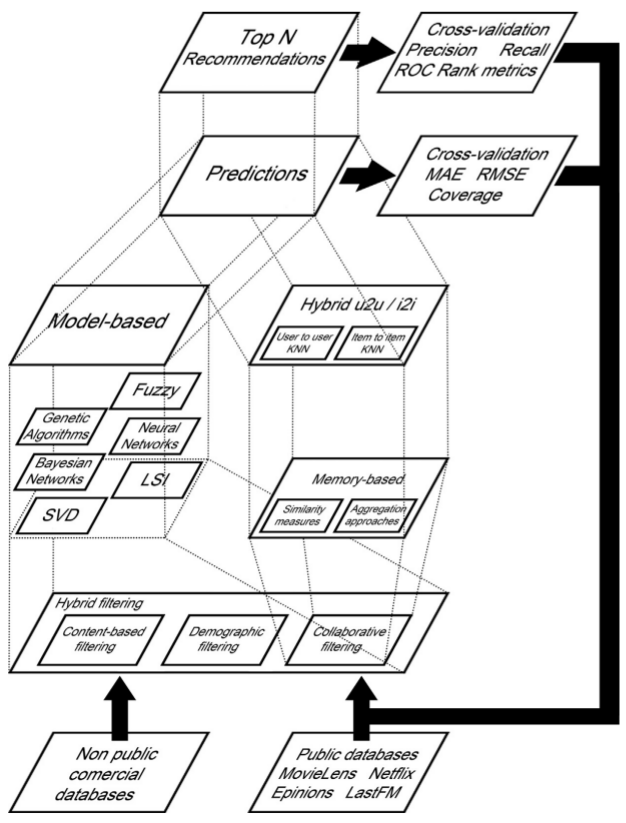
\includegraphics[scale=0.40]{images/model-recomm.png}
	\caption{Modelli di Raccomandazione \cite{Bobadilla:2013:RSS:2483330.2483573}}
	\label{model-rec}
\end{figure}

E' utile citare i metodi di riduzione basati sulla Matrix Factorization, la tecnica model-based Latent Semantic Index (LSI), il metodo di riduzione Singular Value Decomposition
(SVD) e le tecniche di clustering.

Nella Figura \ref{model-rec} viene illustrato un diagramma con le tecniche principali e gli algoritmi di raccomandazione maggiormente utilizzati in letteratura \cite{Bobadilla:2013:RSS:2483330.2483573}.

\subsubsection{Metriche di Valutazione}
La qualità di un sistema di raccomandazione può essere valutata dai risultati forniti in output. Le tipologie di metriche usate, dipendono dal tipo di CF usato. Le metriche possono essere categorizzate in:
Predictive Accuracy, come ad esempio il Mean Absolute Error
(MAE) e sue varianti; Classification Accuracy metrics, come la precision, recall, F1-measure, e sensibilità ROC; Rank Accuracy, come il Mean Average Precision (MAP), e così via.
Desideriamo concentrarci sulla metrica \textbf{Root Mean Squared Error} (RMSE). Infatti la radice quadrata dell'errore quadratico medio, è una metrica molto utilizzata per la raccomandazione di film.

\[ RMSE=\sqrt{\frac{1}{n}\sum_{{i,j}}(p_{i,j}-r_{i,j})^2} \]

dove $n$ è il numero totale dei voti assegnati dagli utenti,$p_{i,j}$ è il voto predetto per l'utente $i$ sull'elemento $j$, ed $r_{i,j}$ è il voto attuale. L'RMSE consente di valutare in maniera precisa i contributi degli errori assoluti tra i valori predetti ed i valori reali \cite{Su:2009:SCF:1592474.1722966}.
 
\subsubsection{Introduzione alla Matrix Factorization}
I modelli di Matrix Factorization possono essere utilizzati per ricercare quali sono i fattori latenti che caratterizzano le interazioni tra due tipologie di entità., tale che le interazioni user-item siano modellate come prodotti interni nello spazio. Ad esempio, due utenti potrebbero votare un determinato film con un voto alto, se ad entrambi piacciono gli attori, o il genere del film, ecc. Quindi, se si riescono a scoprire quali sono i fattori latenti dietro la scelta di un utente, si riesce anche a predire un voto o una possibile preferenza di un altro film rispetto all'utente, perchè le feature associate all'utente dovrebbero convergere alle feature associate all'elemento.

Analizziamo la tecnica dal punto di vista matematico. Sia $U$ l'insieme degli utenti, e sia $D$ l'insieme degli elementi. Sia $R$ la matrice dei voti assegnati dagli utenti agli utenti, di dimensione $\lvert U\rvert\times\lvert D\rvert$. Supponiamo di voler cercare i $K$ fattori latenti. Innanzi tutto bisogna cercare le due matrici, $P$ (una matrice $\lvert U\rvert\times K$) e $Q$ (una matrice $\lvert D\rvert\times K$) tale che il loro prodotto sia una stima del tipo: $R\approx P\times Q^T=\hat{R}$. Ogni riga di $P$ rappresenta il grado di associazione tra un utente e le feature, mentre ogni riga di $Q$ tra un elemento e le feature. Al fine di poter calcolare la predizione di un rating su un elemento $d_j$ votato dall'utente $u_i$, definiamo il prodotto interno tra i due vettori corrispondenti come:
\[\hat{r_{i,j}}={p_i}^Tq_j=\sum_{1}^{k}p_{ik}q_{kj}\]

Quindi un modo per ovviare a questo problema consiste nell'inizializzare le due matrici con alcuni valori, e calcolare la differenza tra i valori stimati ed i valori reali, e infine minimizzare questa differenza in maniera iterativa. Un metodo per minimizzare l'errore calcolato può essere l'algoritmo di discesa del gradiente stocastico oppure l'algoritmo \textbf{Alternating Least Squares} (ALS) \cite{Takacs:2008:MFN:1454008.1454049}.

In generale, mentre l'algoritmo della discesa del gradiente stocastico è più semplice e più veloce di ALS, ALS risulta essere preferibile in molteplici casi, tra cui la parallelizzazione computazionale. In ALS infatti, il sistema calcola ogni vettore $d_j$ indipendentemente dagli altri elementi, così come accade per $u_i$. Ciò comporta un incremento della parallelismo a livello computazionale.

\subsection{Introduzione al Data Stream Processing}
Di recente, è nata una nuova classe di applicazioni \textit{data-intensive}, nei quali i dati vengono modellati come relazioni transienti piuttosto che persistenti. Definiamo con il termine Data Stream, una sequenza di elementi codificati in digitale rappresentanti un'informazione. Esempi di applicazioni \textbf{Data Stream} vanno dal campo finanziario, monitoraggio del traffico di rete, applicazioni web, sicurezza, telecomunicazioni, gestione dati e reti di sensori. Nel modello Data Stream, i dati possono essere tuple relazionali, come ad esempio misurazioni di rete, registro chiamate, pagine web visitate, dati provenienti da sensori, e così via. Tuttavia, questi dati costituiscono un flusso multiplo e tempo variabile, tali da richiedere una nuova tecnologia al fine di poter esser gestiti.

Nei vari scenari applicativi sopra citati, non è efficiente e ne tanto meno semplice gestire i dati in arrivo all'interno di un Database Management System (DBMS) tradizionale. Infatti, i DBMS tradizionali non sono progettati per trattare in maniera rapida un flusso di dati contiguo. Di conseguenza sono nati i Data \textbf{Stream Management System} (DSMS) in grado di gestire un flusso dati continuo. I DSMS sono in grado di offrire un'elevata flessibilità nell'eseguire query continue sullo stream dati. Poichè i DSMS sono data-driven, ogni qualvolta viene eseguita una query, essa produrrà nuovi risultati non appena arrivano nuovi dati da processare.

\begin{figure}[H]
	\centering
	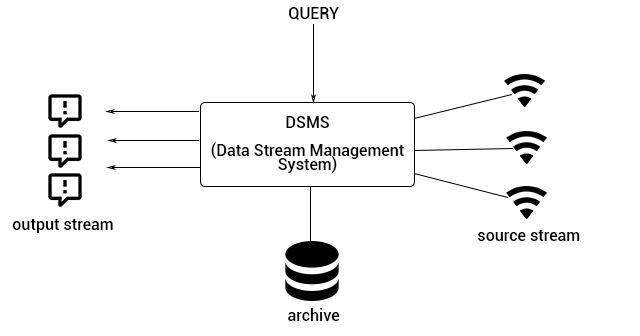
\includegraphics[scale=0.50]{images/dsms.jpg}
	\caption{Architettura DSMS}
	\label{dsms}
\end{figure}

I dati presenti all'interno di uno stream, arrivano online. Il sistema che elabora lo stream, non gestisce l'ordine di arrivo degli elementi da processare. Gli stream inoltre hanno la peculiarità di non avere una dimensione massima prefissata, ma sono altamente variabili. Dopo che il dato è stato processato, o viene scartato, oppure viene archiviato all'interno di uno spazio di storage \cite{Babcock:2002:MID:543613.543615}.

\subsection{Il paradigma Publish-Subscribe}
Il \textbf{Publisher/Subscribe} (pub/sub) è un design pattern, o uno stile architetturale, organizzato in modo che le entità comunicano tra loro in maniera asincrona.

\begin{figure}[H]
	\centering
	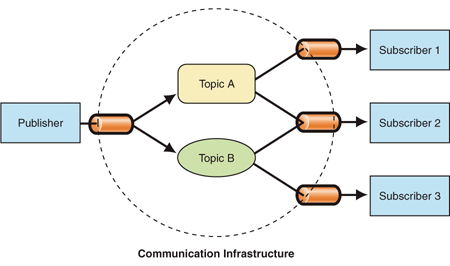
\includegraphics[scale=0.50]{images/pubsub.jpg}
	\caption{Publish/Subscribe}
	\label{pubsub}
\end{figure}

I publisher inviano i messaggi utilizzando un canale di comunicazione denominato topic. I publisher e di subscriber sono generalmente utenti che si sottoscrivono ad uno o più topic, ed in base alla loro posizione gerarchica pubblicheranno/riceveranno le informazioni relative al canale di interesse sottoscritto. Il sistema (vedi Figura \ref{pubsub}) infatti ha il compito di distribuire i messaggi pubblicati dal publisher, a tutti i subscriber iscritti al topic. Infatti quando viene consegnato un nuovo messaggio su un determinato topic, ed un subscriber è iscritto a quest ultimo, il sub sarà notificato con un evento.

\subsection{Il pattern Facade}
Il design pattern \textbf{Facade}, è un pattern strutturale che consente di fornire un'interfaccia semplice ed unificata, che consente di accedere ai diversi sottosistemi dotati di interfacce complesse e diverse tra loro.

\begin{figure}[H]
	\centering
	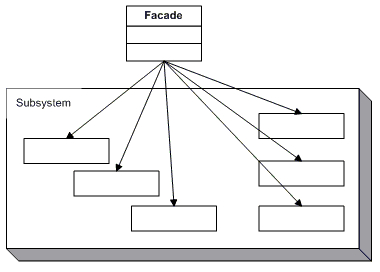
\includegraphics[scale=0.70]{images/facade.jpg}
	\caption{Diagramma UML del Pattern Facade}
	\label{facade}
\end{figure}

Le classi e gli oggetti definiti in questo pattern sono:
\begin{itemize}
\item \textbf{Facade}
\begin{itemize}
	\item Conosce le classi relative al sottosistema che sono responsabili di una richiesta.
	\item Delega le richieste del client all'oggetto del sottosistema appropriato.
\end{itemize}
\item \textbf{Classi del sottosistema}
\begin{itemize}
	\item Implementa le funzionalità di un sottosistema.
	\item Gestisce i compiti assegnati dall'interfaccia \textit{Facade}.
	\item Nasconde la complessità ed i dettagli realizzativi con l'oggetto \textit{Facade}.
\end{itemize}
\end{itemize}

\subsection{Il pattern Singleton}
Il \textbf{Singleton} è un design pattern creazionale che ha lo scopo di garantire che di una determinata classe venga creata una ed una sola istanza, e di fornire un punto di accesso globale a tale istanza.

\begin{figure}[H]
	\centering
	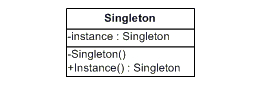
\includegraphics[scale=0.90]{images/singleton.jpg}
	\caption{Diagramma UML del Pattern Singleton}
	\label{singleton}
\end{figure}

Le classi e gli oggetti definiti in questo pattern sono:
\begin{itemize}
	\item \textbf{Singleton}
	\begin{itemize}
		\item Garantisce che un sistema istanzi un massimo di un oggetto di una classe.
		\item Consente al client di accedere all'unica istanza creata.
	\end{itemize}
\end{itemize}

\subsection{Il pattern Model-View-Controller (MVC)}
Il pattern MVC è un pattern architetturale in grado di separare i dati dell'applicazione (contenuti nel Modello) dai componenti per la presentazione grafica (Vista) e la
logica per l'elaborazione dell'input (Controllore).

\begin{figure}[H]
	\centering
	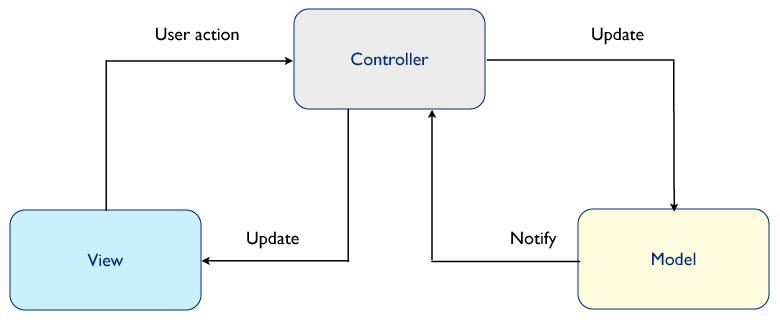
\includegraphics[scale=0.40]{images/mvc.jpg}
	\caption{Il pattern MVC}
	\label{mvc}
\end{figure}

\begin{itemize}
\item \textbf{Model}
\begin{itemize}
	\item Contiene le funzionalità di base ed i dati.
	\item Incapsula lo stato dell'applicazione.
	\item Mostra le funzionalità dell'applicazione.
	\item Notifica alla View i cambiamenti.
	\item Risponde alle query sullo stato. 
\end{itemize}
\item \textbf{View}
\begin{itemize}
	\item Mostra le informazioni all'utente.
	\item Interpreta il Model.
	\item Richiede aggiornamenti dal Model.
	\item Consente al Controller di selezionare la View.
\end{itemize}
\item \textbf{Controller}
\begin{itemize}
	\item Incapsula il comportamento dell'applicazione.
	\item Mappa gli input dell'utente agli aggiornamenti del Model.
	\item Seleziona la View dopo un input.
\end{itemize}
\end{itemize}
Separando il Model dalla View e dal Controller, si da la possibilità di associare più View allo stesso Model. Nel caso in cui l'utilizzatore modifica i dati contenuti nel Model mediante il Controller di una determinata
View, tutte le altre View ricollegate a quel model ne propagano la variazione.

\subsection{La tecnologia WebSocket}
Il protocollo WebSocket standardizzato dall'IETF come RFC 6455 consente la comunicazione bidirezionale e full duplex mediante una singola connessione TCP. La connessione persistente, viene instaurata mediante un sistema di handshaking client-key ed un modello di sicurezza origin-based. L'obiettivo di questa tecnologia è fornire un meccanismo per quelle applicazioni web-based che necessitano di comunicare con server che non consentono di aprire connessioni HTTP multiple (ad esempio usando XMLHttpRequest, o <iframe>, o un sistema di polling), oppure per motivi di sicurezza per quei sistemi che bloccano l'utilizzo di porte non standard mediante firewall.

\begin{figure}[H]
	\centering
	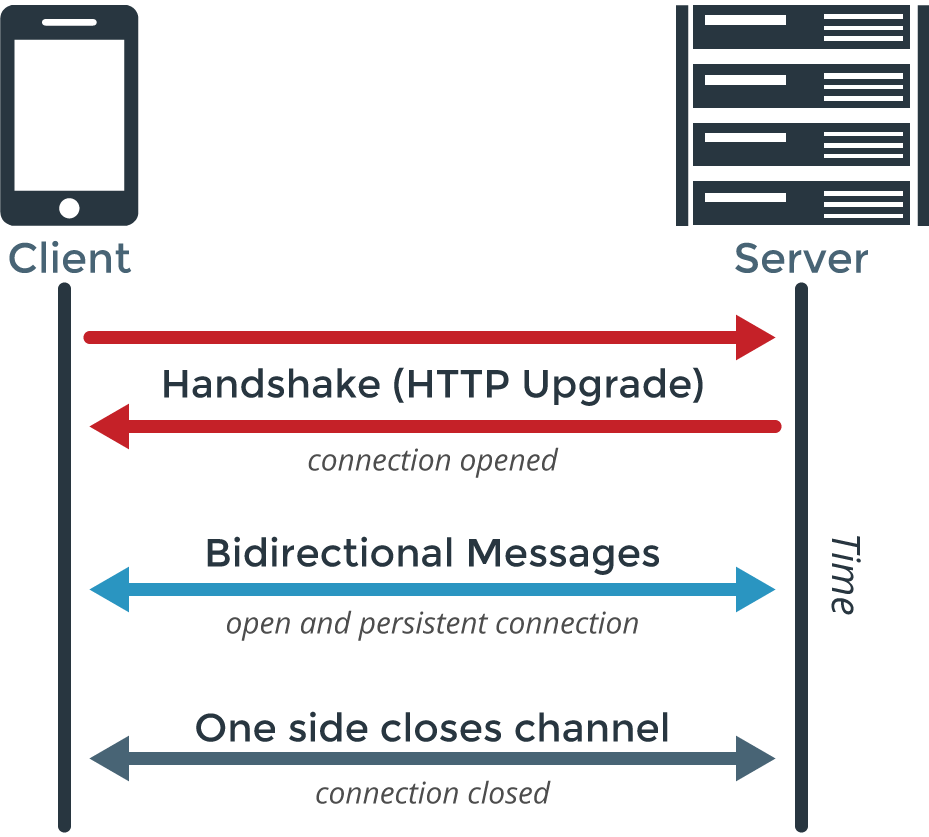
\includegraphics[scale=0.25]{images/websocket.png}
	\caption{La tecnologia WebSocket}
	\label{websocket}
\end{figure}

Il protocollo WebSocket viene inizializzato in primis con una fase di handshake e successivamente si procede con il trasferimento dati. Le porte di comunicazione utilizzate sono le stesse porte TCP di HTTP (80) e HTTPS (443). Inoltre vengono riutilizzati gli stessi elementi strutturali di HTTP, quali proxy ed autenticazione.

\begin{figure}[H]
	\centering
	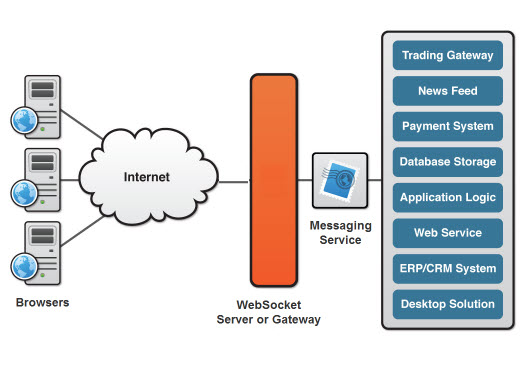
\includegraphics[scale=1.00]{images/websocket-architecture.jpg}
	\caption{Architettura di WebSocket}
	\label{websocket-architecture}
\end{figure}

Infine lo schema URI utilizzato è \texttt{ws://} per connessioni in chiaro, \texttt{wss://} per connessioni cifrate con TLS\cite{fette2011websocket}.

WebSocket viene utilizzato molto spesso per ottenere una comunicazione che sia a bassa latenza, efficiente e quasi realtime tra client e server. Vari scenari applicativi sono costituiti da giochi online multiplayer, chat, aggiornamento in tempo reale di informazioni e così via.

\section{Soluzione proposta}

\subsection{La libreria Spark}

Apache Spark è un sistema di cluster computing di tipo general-purpose, scalabile e veloce. Dispone di API di alto livello in \textbf{Java}, \textbf{Scala},\textbf{ Python} ed \textbf{R}, e un engine ottimizzato che supporta grafi di esecuzione generici. Integra inoltre un ampio set di tool come \textbf{Spark SQL}, per structured data processing, \textbf{MLlib} per il machine learning e \textbf{Spark Streaming}, descritti nelle sezioni successive. Spark è eseguibile sia su sistemi Windows che UNIX-like (Linux, Mac OS) \cite{spark}. \\

Una delle possibili configurazioni di un sistema Spark è la modalità \textit{cluster}, mostrata in Figura \ref{spark-cluster}. 

\begin{figure}[H]
	\centering
	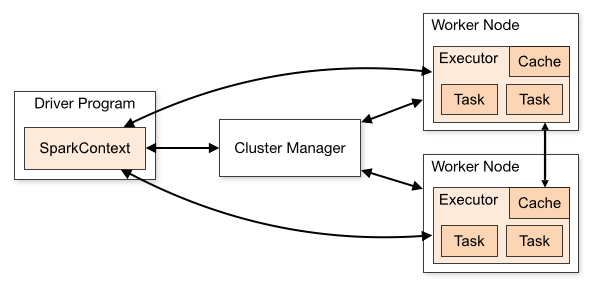
\includegraphics[scale=0.50]{images/cluster-overview.png}
	\caption{Configurazione in Spark di tipo Cluster Mode \cite{spark}}
	\label{spark-cluster}
\end{figure}

Le applicazioni Spark sono eseguite come un set di processi indipendenti sul cluster, coordinati dall'oggetto \textit{SparkContext} del programma sorgente (detto \textbf{driver program}). Precisamente, il programma driver può connettersi su diversi tipi di \textit{cluster managers} (ad esempio un cluster di tipo Standalone, Mesos o YARN), il quale alloca le risorse a disposizione delle applicazioni. Una volta connesso, Spark scansiona i nodi del cluster alla ricerca degli \textbf{executor} (detti anche \textit{worker node}), i quali eseguono effettivamente i task e il data storage delle applicazioni. A questo punto il driver invia il codice dell'applicazione agli executor (tipicamente un file JAR o Python incluso nello SparkContext) e schedula i task per l'esecuzione parallela \cite{spark}. 

Alcune considerazioni riguardo tale architettura sono: 
\begin{itemize}
	\item Ogni applicazione gestisce i propri workers, i quali restano attivi durante tutto il ciclo di vita ed eseguono task multipli in thread multipli. Questo implica un isolamento tra le applicazioni, sia lato scheduling (ogni driver schedula i propri tasks) sia lato executor (tasks relativi ad applicazioni differenti risiedono in JVM differenti). Tuttavia ciò implica che non è possibile condividere nativamente i dati tra applicazioni diverse, a meno di utilizzare uno storage system esterno;
	\item Il driver deve poter gestire le connessioni con i workers durante l'intero ciclo di vita dell'applicazione. Per questo motivo dev'essere sempre garantita la visibilità a livello di rete tra driver e workers durante l'esecuzione;
	\item \`E necessario che driver e worker abbiano, a livello di rete, una distanza relativamente breve, preferibilmente nella stessa LAN, affinché lo scheduling sia rapidamente eseguito \cite{spark}. 
\end{itemize}

Il principio di funzionamento di Spark si basa sostanzialmente sul concetto di \textit{Resilient Distributed Dataset} (\textbf{RDD}). Un RDD è una collezione di dati su cui è possibile operare parallelamente, ed è distribuita su tutti i nodi del cluster come file system Hadoop oppure è generata da una collezione esistente in Java o Scala \cite{spark}. \\

Una seconda astrazione è rappresentata dalle variabili condivise (\textit{shared variables}), utilizzate nelle computazioni parallele. Di default Spark tiene traccia delle variabili istanziate nei vari task, e consente se necessario di condividerle fra task o fra task e driver. Le variabili condivise possono essere di due tipi: di tipo \textit{broadcast}, il cui valore viene salvato nella cache per ogni nodo, e di tipo \textit{accumulatore}, per esempio contatori o sommatori \cite{spark}.

\subsubsection{Spark Streaming}

Spark Streaming è un'estensione delle Core API di Spark per lo\textbf{ stream processing} di live data streams ad alto throughput. Supporta molteplici sorgenti di data stream come\textbf{ Kafka}, Flume, Twitter, ZeroMQ, Kinesis o socket TCP, i quali possono essere processati tramite direttive come \textit{map}, \textit{join}, \textit{reduce} e \textit{window}. Nel post processing è possibile salvare i data stream in un file system, in un database o visualizzarli in una live dashboard. Come ulteriore fase nella pipeline di operazione rientra anche il machine learning ed il graph processing. In Figura \ref{spark-streaming} viene riassunta l'architettura descritta \cite{spark}. 

\begin{figure}[H]
	\centering
	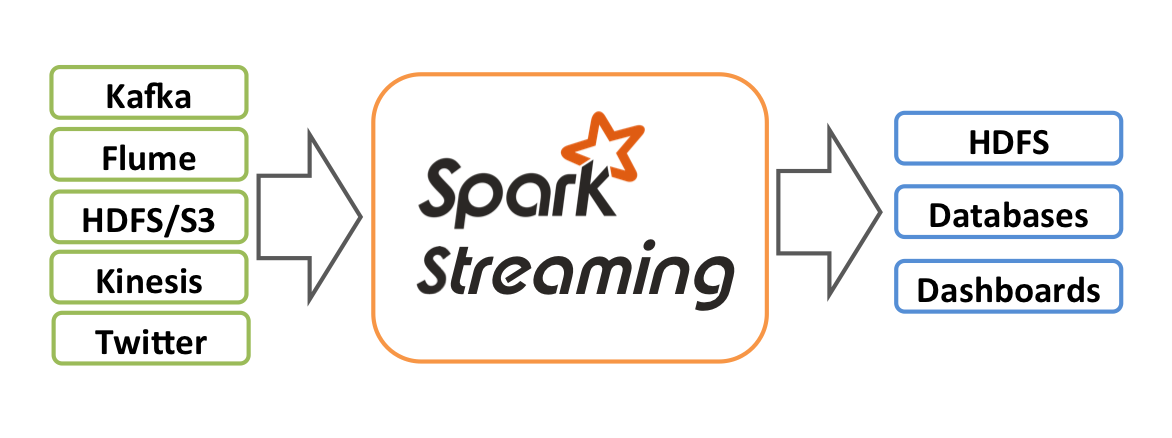
\includegraphics[scale=0.50]{images/streaming-arch.png}
	\caption{Architettura di Spark Streaming \cite{spark}}
	\label{spark-streaming}
\end{figure}

Nello specifico, i data streams ricevuti vengono suddivisi in frammenti (\textit{batches}), processati da Spark per generare lo stream finale risultante in batches, come mostrato in Figura \ref{spark-streaming-processing} \cite{spark}.

\begin{figure}[H]
	\centering
	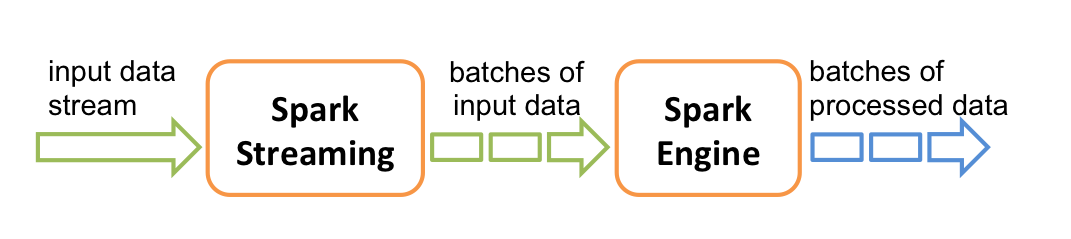
\includegraphics[scale=0.50]{images/streaming-flow.png}
	\caption{Spark Streaming Data Stream Processing \cite{spark}}
	\label{spark-streaming-processing}
\end{figure}

A livello alto il flusso continuo di dati è rappresento da una struttura astratta detta \textit{discretized stream} o \textit{DStream}, il cui contenuto è rappresentato da tutte le sorgenti collegate eventualmente con Spark, o da stream risultati da altri DStream. Internamente, un DStream è rappresentato tramite una sequenza di RDD \cite{spark}. 

\subsubsection{Spark MLlib}

Spark MLlib è la libreria per il machine learning di Spark, ed il suo obiettivo è di rendere l'uso di tali funzionalità semplice e scalabile. Comprende i più comuni algoritmi di learning quali classificazione, regressione, clustering, filtro collaborativo, riduzione dello spazio delle features, etc. \cite{spark}. 

\subsubsection{Spark SQL}

Spark SQL è un modulo di Spark per il processing di dati strutturati. A differenza delle API RDD la sua interfaccia consente di descrivere in maniera dettagliata la struttura e le operazioni da eseguire sui dati, in stile SQL. Le strutture astratte di riferimento per questo modulo sono i \textbf{Dataframes} e i \textbf{Datasets} \cite{spark}.\\

Un \textbf{Dataframe} è un collezione distribuita di informazioni organizzata in colonne e attributi. Concettualmente è equivalente ad una tabella in un database relazionale, con caratteristiche aggiuntive fornite da Spark. In accordo con tale definizione sono presenti, oltre alle classiche funzionalità SQL, la creazione di DataFrame a partire da un RDD o un oggetto JSON e viceversa \cite{spark}.\\

Un \textbf{Dataset} invece è un'interfaccia sperimentale introdotta nella versione 1.6 di Spark, mirata all'integrazione delle API RDD con l'engine SQL. Attualmente il supporto è limitato alle API Java e Scala \cite{spark}.

\subsection{Apache Kafka}

Apache Kafka è un sistema di messaggistica di tipo publish-subscribe, orientato alla distribuzione. La sua architettura consente ad un singolo cluster di agire da backbone centrale per i dati di grandi organizzazioni, e gli stream vengono partizionati e distribuiti lungo tutti i nodi del cluster, sfruttando la potenza di calcolo di ogni singola macchina. Di seguito si introduce la terminologia utilizzata in Kafka: 

\begin{itemize}
	\item Kafka organizza i flussi dei messaggi in categorie chiamate \textit{topics};
	\item I processi che si occupano di pubblicare i messaggi in Kafka sono chiamati \textit{producers};
	\item I processi che effettuano una sottoscrizione ad un topic ed elaborano i messaggi pubblicati sullo stesso sono chiamati \textit{consumers};
	\item I nodi all'interno del cluster(producers e consumers) sono coordinati da uno o più server chiamati \textit{brokers} \cite{kafka}.
	
\end{itemize}

A livello concettuale il funzionamento di Kafka è riassunto in Figura \ref{kafka}. La comunicazione tra client e server avviene tramite protocollo TCP. Sono presenti varie implementazioni del client Kafka, disponibili in vari linguaggi tra cui Java, Javascript e PHP \cite{kafka}. 

\begin{figure}[H]
	\centering
	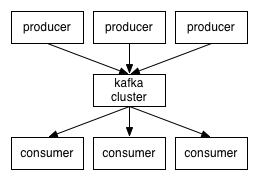
\includegraphics[scale=0.80]{images/kafka.png}
	\caption{Architettura di Apache Kafka \cite{kafka}}
	\label{kafka}
\end{figure}


Di seguito viene mostrata nel dettaglio la struttura di un topic in Figura \ref{kafka-topic}. Per ogni topic Kafka effettua un partizionamento dei messaggi in arrivo, tenendo traccia dell'ordine di arrivo con un sistema di log \cite{kafka}. 

\begin{figure}[H]
	\centering
	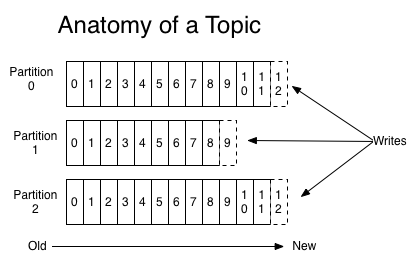
\includegraphics[scale=0.80]{images/log_anatomy.png}
	\caption{Struttura di un topic in Kafka \cite{kafka}}
	\label{kafka-topic}
\end{figure}

Ogni partizione è una sequenza immutabile di messaggi, registrata e ordinata in un commit log. Ad ogni messaggio presente viene assegnato un id sequenziale, detto \textit{offset}, che identifica univocamente un messaggio nella relativa partizione \cite{kafka}.

Il cluster di Kafka conserva in memoria tutti i messaggi pubblicati, letti o non dai consumers, per un periodo di tempo configurabile. In pratica, il server registra dei metadati relativi ad ogni posizione del consumer nel log, chiamato appunto offset. Tale offset è fissato dal consumer, il quale può leggere i messaggi nell'ordine preferito \cite{kafka}. 


\subsubsection{Integrazione con Spark Streaming}

Le API di Spark Streaming offrono la possibilità di configurare Kafka come sorgente di data stream, attraverso due possibili approcci \cite{spark}. 

Il primo approccio è detto \textbf{Receiver-based}, e consiste nell'implementazione di un Receiver tramite le API di Kafka. I dati ricevuti attraverso tale oggetto vengono memorizzati e processati nei worker node. Tuttavia, tale approccio potrebbe non garantire la consistenza in caso di data loss, ed è dunque necessario abilitare un meccanismo di integrità chiamato \textit{Ahead Logs} \cite{spark}. \\

Il secondo approccio, detto \textit{Direct Approch} o \textit{Receivers less}, non prevede l'uso di Receivers ma interroga periodicamente il server Kafka per rilevare il topic e la partizione aggiornata di recente, definendo in automatico la dimensione del batch di dati da processare. I vantaggi di questa tecnica sono: 
\begin{itemize}
	\item \textit{Parallelismo semplificato: } Non è necessario creare ed unificare stream multipli di Kafka. Tramite la funzione \textit{directStream}, Spark Streaming effettua un mapping tra le partizioni di Kafka in RDD, semplificandone l'elaborazione in parallelo;
	\item \textit{Efficienza: } Il meccanismo Write Ahead Logs potrebbe generare problemi di duplicazione dei dati e relativi conflitti, nel momento in cui entrambe le istanze di Spark e Kafka tentino di risolvere una perdita di informazioni. Con un approccio diretto senza Receivers tale problema non sussiste \cite{spark}.
\end{itemize}

\subsection{Il framework Node.js}

Node.js è un framework per la realizzazione di applicazioni web in Javascript lato server. La piattaforma è basata sul \textbf{Javascript Engine V8}, il runtime di Google utilizzato anche in Chrome, disponibile per le principali piattaforme, anche se maggiormente performante su sistemi operativi UNIX-like.

\begin{figure}[H]
	\centering
	
\includegraphics[scale=0.50]{images/nodejs.png}
	\caption{Il Framework Node.js}
	\label{node}
\end{figure}

A differenza dei classici web server, che sfruttano un modello a processi concorrenti, Node.js utilizza una modalità di tipo \textit{event-driven} per l'accesso alle risorse. Scrivere un'applicazione in Node.js dunque consiste nel definire una serie di eventi che il sistema operativo deve monitorare, e all'attivazione degli stessi eseguire una funzione associata a tale evento, detta \textbf{callback}. Tale approccio definisce processi non bloccanti, evita il verificarsi di deadlocks, e in generale le operazioni di I/O non avvengono in maniera diretta. Ciò garantisce una maggiore \textbf{scalabilità} e \textbf{flessibilità} dell'architettura web. \\

All'interno del framework si ha a disposizione il package manager \textbf{npm}, tramite il quale è possibile installare moduli e librerie, gestire le diverse release, gli update e le dipendenze.\\

Il modulo \textbf{kafka.node} (\href{https://www.npmjs.com/package/kafka-node}{https://www.npmjs.com/package/kafka-node}) mette a disposizione un client in Node.js per la connessione ad un server Kafka. \`E possibile implementare sia il Producer che il Consumer, gestire gli eventi, creare topics, etc.

\subsection{Angular.js}

L'interfaccia dell'applicazione è stata realizzata attraverso il framework AngularJS, creando un modello MVC che sfrutta il two-way data binding di AngularJS.

\begin{figure}[H]
	\centering
	
\includegraphics[scale=0.50]{images/angular.png}
	\caption{Il Framework Angular.JS}
	\label{angular}
\end{figure}

Il front end è costruito grazie alla libreria Bootstrap, un framework che mira alla creazione di pagine web dinamiche, fluide e adattabili a qualsiasi dispositivo con differenti grandezze e risoluzione, che contiene una serie di modelli CSS, HTML e Javascript dei componenti web maggiormente utilizzati. Altre librerie utilizzate sono: 
\begin{itemize}
	\item \textbf{Angular Route} Una libreria che gestisce le view ed il routing in una macchina a stati.
\end{itemize}

Il layout contiene le seguenti directory: 
\begin{itemize}
	\item \textbf{/css} Fogli di stile per le pagine HTML;
	\item \textbf{/fonts} Web font;
	\item \textbf{/img} Logo e immagini;
	\item \textbf{/vendor} Librerie utilizzate dall'applicazione;
	\item \textbf{/js} File Javascript della dashboard;
	\begin{itemize}
		\item \textbf{/controllers} Script dei controller di AngularJS;
		\item \textbf{views} File HTML relativi alle view di AngularJS;
		\item \textbf{/services} Direttive di AngularJS per gli eventi associati al websocket.
	\end{itemize}
	\item \textbf{app.js} Script principale dell'applicazione. Al suo interno sono definiti gli stati con le relative view, le transizioni e le direttive associate ad ogni view per i relativi dati da visualizzare.
\end{itemize}

\subsection{La libreria Socket.IO}

Socket.io è una libreria Javascript per applicazioni web real time. Abilita una comunicazione di tipo bidirezionale tra client (generalmente eseguito nel browser) e server (applicazione Node.js).\\

Principalmente il protocollo utilizzato è WebSocket, con un modello di esecuzione di tipo asincrono.  

\section{Analisi e progettazione della soluzione proposta}
\subsection {Architettura del sistema}

\subsection {Architettura software}
\lipsum

\subsection {Configurazione del sistema}
Il sistema operativo utilizzato per l'implementazione della soluzione è \textbf{Ubuntu 15.10}. I nodi per testare la soluzione, sono dotati di configurazioni hardware eterogenee.

Suddividiamo in 3 parti la configurazione relativa all'architettura del sistema.
\begin{itemize}
\item {\textbf{Configurazione di Apache Spark in Cluster Mode}}\\\\
In primis occorre scaricare \textbf{Apache Spark} ( \href{http://spark.apache.org/downloads.html}{http://spark.apache.org/downloads.html}). La versione utilizzata è stata la "\textbf{Pre-built for Hadoop 2.6 and later}".
Dopo aver effettuato il download ed aver estratto il contenuto nella propria \texttt{/home}, creiamo una copia del file \texttt{spark-env.sh.template} chiamandolo \texttt{spark-env.sh} all'interno della directory \texttt{conf} della \texttt{root} di Spark. All'interno del file possiamo specificare varie direttive, ma per il nostro scopo settiamo quelle essenziali al corretto funzionamento:
\begin{lstlisting}[language=bash, caption=spark-env.sh]
export SPARK_WORKER_CORES=n
export SPARK_WORKER_MEMORY=mg
export SPARK_MASTER_IP=X.X.X.X
export SPARK_MASTER_PORT=7077
export MASTER=spark://${SPARK_MASTER_IP}:${SPARK_MASTER_PORT}
\end{lstlisting}
La variabile \texttt{SPARK\_WORKER\_CORES}, serve per poter configurare il numero di core da utilizzare sulla macchina (nel nostro caso settiamo il numero massimo di core che vogliamo utilizzare relativi ai nodi Slave).
La variabile \texttt{SPARK\_WORKER\_MEMORY}, consente di specificare quanta memoria dei rispettivi Workers si desidera allocare per l'esecuzione del software (ad esempio 1000m, 2g).
La variabile \texttt{SPARK\_MASTER\_PORT}, consente di specificare la porta sulla quale avviare il nodo Master.
La variabile \texttt{SPARK\_MASTER\_IP}, per impostare l'indirizzo IP o l'hostname del nodo Master.

Dopo aver configurato il nodo Master, avviamolo dal terminale mediante \texttt{/sbin/start-master.sh}.
Successivamente, avviamo i nodi Worker mediante \texttt{/sbin/start-slave.sh spark://SPARK\_MASTER\_IP:SPARK\_MASTER\_PORT}.
Dal nodo Master, possiamo aprire il browser, digitando \texttt{http://localhost:SPARK\_MASTER\_PORT} in modo da visualizzare dalla Dashboard i Worker connessi ed i Job avviati nel sistema.
Infine se il sistema non è configurato con \texttt{hadoop}, configurare i percorsi ed i relativi file anche sui Worker.

\item {\textbf{Configurazione di Apache Kafka}}\\\\
Come prima cosa occorre scaricare \textbf{Apache Kafka} ( \href{http://kafka.apache.org/downloads.html}{http://kafka.apache.org/downloads.html}). La versione utilizzata è la \textbf{0.9.0.1} per \textbf{Scala 2.10}, quindi \textbf{kafka\_2.10-0.9.0.1}. Dopo aver effettuato il download ed aver estratto il contenuto nella propria \texttt{/home}, apriamo il \texttt{server.properties} all'interno della directory \texttt{config} della \texttt{root} di Spark.

All'interno del file, aggiungiamo le seguenti stringhe nel caso in cui non dovessero essere presenti: 
\begin{lstlisting}[language=bash,caption=server.properties]
zookeeper.connect=localhost:2181
advertised.host.name=hostname/ip
\end{lstlisting}
La stringa \texttt{zookeeper.connect=localhost:2181} consente di specificare i parametri di connessione nel formato \texttt{hostname:port} dove \texttt{host} e \texttt{port} rappresentano rispettivamente l'hostname e la porta del server \textbf{ZooKeeper}. La stringa \texttt{advertised.host.name} se settata, rappresenta l'hostname che verrà fornito ai broker, producer, e consumer per connettersi ad esso.
Successivamente verranno illustrati quali sono le operazioni per creare i topic ed avviare il server Zookeeper da terminale.

\item {\textbf{Configurazione del Framework Node.js}}\\\\
Dal terminale di Ubuntu, digitare \texttt{sudo apt-get install nodejs, npm}, per installare NodeJS ed il gestore dei pacchetti per Javascript \texttt{npm}. Successivamente creiamo un link simbolico per node in questo modo \texttt{sudo ln -s /usr/bin/nodejs /usr/bin/node}. Accertiamoci inoltre con \texttt{node -v} che la versione di node sia la \textbf{5.10.1} (nel caso in cui la versione non dovesse essere questa, sarà necessario effettuare un ulteriore upgrade/downgrade).
Dopo aver configurato l'ambiente di lavoro, è necessario effettuare il download della applicazione ed estrarla nella directory desiderata (ad esempio \texttt{kafka\_socket}).
Dal terminale, entrare all'interno della directory \texttt{kafka\_socket} ed effettuare l'installazione di tutte le dipendenze richieste dall'applicazione mediante \texttt{sudo npm install -g}.
Nel punto successivo, sarà illustrato come avviare l'applicazione Node.js.
\item {\textbf{Avvio del Sistema}}\\\\
Lanciamo il seguente script dal terminale mediante \texttt{sudo ./start.sh}.

\begin{lstlisting}[language=bash,caption=start.sh]
#!/bin/bash
SCALA_VERSION="2.10"
KAFKA_VERSION="0.9.0.1"

#Directory Path of NodeJS Script
NODE_SCRIPT_DIR="kafka_socket"

#I supposed that Kafka Installation Directory is located in /home/<user>
KAFKA_HOME=$HOME/kafka_$SCALA_VERSION-$KAFKA_VERSION

#Start Zookeeper and Kafka Server as daemon
echo "Starting Zookeeper and Kafka Server..."
$KAFKA_HOME/bin/zookeeper-server-start.sh -daemon $KAFKA_HOME/config/zookeeper.properties
sleep 5
$KAFKA_HOME/bin/kafka-server-start.sh -daemon $KAFKA_HOME/config/server.properties
sleep 5

#Create Topics
echo "Creating Topics..."
$KAFKA_HOME/bin/kafka-topics.sh --create --zookeeper localhost:2181 --replication-factor 1 --partitions 1 --topic votes
$KAFKA_HOME/bin/kafka-topics.sh --create --zookeeper localhost:2181 --replication-factor 1 --partitions 1 --topic result

#Start node.js App
echo "Starting App on localhost:3000"
node $HOME/$NODE_SCRIPT_DIR/app.js --port 3000
\end{lstlisting}
Lo script è stato realizzato per automatizzare la configurazione dell'ambiente di lavoro. Leggendo lo script si intuisce che sia Zookeeper che Kafka Server vengono lanciati come demoni. Inoltre i topic creati mediante \texttt{kafka-topics.sh} presente all'interno della cartella \texttt{bin} della \texttt{root} di Kafka sono rispettivamente: \textbf{votes}, \textbf{result}. Il primo topic viene utilizzato per inviare i voti degli utenti, mentre il topic result, per fornire i risultati derivanti dal filtro collaborativo.
Infine possiamo notare come l'applicazione Node.js venga avviata in locale sulla porta 3000.

\end{itemize}


\section{Conclusioni e sviluppi futuri}

\clearpage
\addcontentsline{toc}{section}{Bibliografia}
\nocite{*}
\bibliographystyle{plain}
\bibliography{biblib}

\newpage
\section{Sorgenti}
\begin{appendices}
	\section{Sorgenti Spark}
	\begin{lstlisting}[style=scalacode, caption=Main.scala]
package ml

import cep.CEP
import commons.{FileParser, KafkaCommons, SparkCommons}
import org.apache.log4j.{Level, Logger}

/**
*
* @authors Mauro Losciale and Pietro Tedeschi.
*/
object Main {

def main(args: Array[String]): Unit ={

Logger.getLogger("org.apache.spark").setLevel(Level.ERROR)
Logger.getLogger("org.eclipse.jetty.server").setLevel(Level.OFF)

val ratings = FileParser.parseRatings()
val movies = FileParser.parseMovies()

val numRatings = ratings.count()
val numUsers = ratings.map(_._2.user).distinct().count()
val numMovies = ratings.map(_._2.product).distinct().count()

println("Got " + numRatings + " ratings from "
+ numUsers + " users on " + numMovies + " movies.")

val messages = KafkaCommons.kafkaDirectStreaming()

messages.foreachRDD { rdd =>
val votes = rdd.map(_._2)
val tableVotes = SparkCommons.sqlContext.read.option("header","true")
	.option("inferSchema","true")
	.json(votes).toDF().na.drop()

if (tableVotes.count() > 0) {

tableVotes.show()
tableVotes.registerTempTable("tableVotes")

val query = SparkCommons.sqlContext.sql("SELECT * FROM tableVotes WHERE rating > 3")
CEP.hasEnoughVotes(query, tableVotes, ratings, movies)

} else println("Nessun voto ricevuto")


}

SparkCommons.ssc.start()
SparkCommons.ssc.awaitTermination()

}

}
	\end{lstlisting}
	\begin{lstlisting}[style=scalacode, caption=SparkCommons.scala]
		package commons
		
		import org.apache.spark.sql.SQLContext
		import org.apache.spark.streaming._
		import org.apache.spark.{SparkConf, SparkContext}
		
		/**
		* Handles configuration, context and so
		*
		* @authors Mauro Losciale and Pietro Tedeschi.
		*/
		object SparkCommons {
		//build the SparkConf  object at once
		lazy val conf = {
		new SparkConf(false)
		.setMaster("local[*]")
		.setAppName("Collaborative Filtering with Kafka")
		.set("spark.logConf", "true")
		}
		
		lazy val sc = SparkContext.getOrCreate(conf)
		lazy val ssc = new StreamingContext(sc, Seconds(30))
		lazy val sqlContext = new SQLContext(sc)
		
		sc.addJar("target/scala-2.10/mlspark-assembly-1.0.jar")
		}
	\end{lstlisting}
	
	\begin{lstlisting}[style=scalacode, caption=KafkaCommons.scala]
		package commons
		
		import java.util.Properties
		
		import kafka.producer.{Producer, ProducerConfig}
		import kafka.serializer.StringDecoder
		import org.apache.spark.streaming.Seconds
		import org.apache.spark.streaming.kafka.{KafkaUtils, OffsetRange}
		
		/**
		*
		* @authors Mauro Losciale and Pietro Tedeschi.
		*/
		object KafkaCommons {
		
		val kafkaTopics = "votes"    // command separated list of topics
		val kafkaBrokers = "makaveli-desktop:9092"
		var offsetRanges = Array[OffsetRange]()
		val kafkaParams = Map[String, String]("metadata.broker.list" -> kafkaBrokers
		)
		val topicsSet = kafkaTopics.split(",").toSet
		val messages = KafkaUtils.createDirectStream[String, String, StringDecoder, StringDecoder](
		SparkCommons.ssc, kafkaParams, topicsSet)
		
		val props:Properties = new Properties()
		props.put("metadata.broker.list", "192.168.0.4:9092")
		props.put("serializer.class", "kafka.serializer.StringEncoder")
		
		val config = new ProducerConfig(props)
		val producer = new Producer[String, String](config)
		
		def kafkaDirectStreaming() = {
		
		KafkaUtils.createDirectStream[String, String, StringDecoder, StringDecoder](
		SparkCommons.ssc, kafkaParams, topicsSet).window(Seconds(60), Seconds(30))
		}
		
		}
		
	\end{lstlisting}
	\begin{lstlisting}[style=scalacode, caption=CollaborativeFiltering.scala]
		package ml
		
		import commons.{KafkaCommons, SparkCommons}
		import kafka.producer.{KeyedMessage, Producer}
		import org.apache.spark.mllib.recommendation.{ALS, MatrixFactorizationModel, Rating}
		import org.apache.spark.rdd._
		import org.json4s.JsonDSL._
		import org.json4s.jackson.JsonMethods._
		
		/**
		*
		* @authors Mauro Losciale and Pietro Tedeschi.
		*/
		object CollaborativeFiltering {
		
		def userCF(rdd: RDD[Rating], ratings: RDD[(Long, Rating)], movies: Map[Int, String]) = {
		
		val myRatingsRDD = rdd
		
		// split ratings into train (60%), validation (20%), and test (20%) based on the
		// last digit of the timestamp, add myRatings to train, and cache them
		
		val numPartitions = 4
		
		val training = ratings.filter(x => x._1 < 6)
		.values
		.union(myRatingsRDD)
		.repartition(numPartitions)
		.cache()
		
		val validation = ratings.filter(x => x._1 >= 6 && x._1 < 8)
		.values
		.repartition(numPartitions)
		.cache()
		
		val test = ratings.filter(x => x._1 >= 8).values.cache()
		
		val numTraining = training.count()
		val numValidation = validation.count()
		val numTest = test.count()
		
		println("Training: " + numTraining + ", validation: " + numValidation + ", test: " + numTest)
		
		// train models and evaluate them on the validation set
		
		val ranks = List(8, 12)
		val lambdas = List(0.1, 10.0)
		val numIters = List(10, 20)
		var bestModel: Option[MatrixFactorizationModel] = None
		var bestValidationRmse = Double.MaxValue
		var bestRank = 0
		var bestLambda = -1.0
		var bestNumIter = -1
		for (rank <- ranks; lambda <- lambdas; numIter <- numIters) {
		val model = ALS.train(training, rank, numIter, lambda)
		val validationRmse = computeRmse(model, validation, numValidation)
		println("RMSE (validation) = " + validationRmse + " for the model trained with rank = "
		+ rank + ", lambda = " + lambda + ", and numIter = " + numIter + ".")
		if (validationRmse < bestValidationRmse) {
		bestModel = Some(model)
		bestValidationRmse = validationRmse
		bestRank = rank
		bestLambda = lambda
		bestNumIter = numIter
		}
		}
		
		// evaluate the best model on the test set
		
		val testRmse = computeRmse(bestModel.get, test, numTest)
		
		println("The best model was trained with rank = " + bestRank + " and lambda = " + bestLambda
		+ ", and numIter = " + bestNumIter + ", and its RMSE on the test set is " + testRmse + ".")
		
		// make personalized recommendations
		
		val myRatedMovieIds = myRatingsRDD.map(_.product).collect().toSet
		val candidates = SparkCommons.sc.parallelize(
			movies.keys.filter(!myRatedMovieIds.contains(_)).toSeq)
		val recommendations = bestModel.get
		.predict(candidates.map((0, _)))
		.collect()
		.sortBy(-_.rating)
		.take(9)
		
		out(recommendations, movies, KafkaCommons.producer)
		
		}
		
		/** Compute RMSE (Root Mean Squared Error). */
		def computeRmse(model: MatrixFactorizationModel, data: RDD[Rating], n: Long): Double = {
		val predictions: RDD[Rating] = model.predict(data.map(x => (x.user, x.product)))
		val predictionsAndRatings = predictions.map(x => ((x.user, x.product), x.rating))
		.join(data.map(x => ((x.user, x.product), x.rating)))
		.values
		math.sqrt(predictionsAndRatings.map(x => (x._1 - x._2) * (x._1 - x._2)).reduce(_ + _) / n)
		}
		
		/** Write recommendations array to a JSON file **/
		def out(data: Array[Rating], film: Map[Int, String], producer: Producer[String, String]) = {
		
		println("Movies recommended for you:")
		
		data.foreach { r =>
		
		val jsonVote = ("movieid", r.product) ~("rating", r.rating.toInt) ~("title", film(r.product))
		producer.send(new KeyedMessage[String, String]("result", compact(render(jsonVote)).toString))
		}
		}
		}
		
	\end{lstlisting}
	\begin{lstlisting}[style=scalacode, caption=CEP.scala]
		package cep
		
		import ml.CollaborativeFiltering
		import org.apache.spark.mllib.recommendation.Rating
		import org.apache.spark.rdd.RDD
		import org.apache.spark.sql.DataFrame
		
		/**
		*
		* @authors Mauro Losciale and Pietro Tedeschi.
		*/
		object CEP {
		
		def hasEnoughVotes(query: DataFrame, table: DataFrame, ratings: RDD[(Long,Rating)], movies: Map[Int, String]) = {
		
		query.count() match {
		
			case c if c == 0 => println("Nessun voto valido")
			case c if c > 3 =>
				val votesRating = table.map(v => Rating(0, v(0).toString.toInt, v(1).toString.toDouble))
				println("Make CF")
				CollaborativeFiltering.userCF(votesRating, ratings, movies)
			case c if c <= 3 => println("Voti validi inferiori a 4")
				}
			}
		
		}
		
	\end{lstlisting}
	\section{Sorgenti Node.js}
	
	\begin{lstlisting}[language=Javascript, caption=app.js]
		var vote_server = require('./lib/vote_server');
		var kafka_consumer = require('./lib/kafka_consumer');
		var kafka_producer = require('./lib/kafka_producer');
		var http = require('http');
		var express = require('express');
		var path = require('path');
		var argv = require('minimist')(process.argv.slice(2));
		
		var favicon = require('serve-favicon');
		var logger = require('morgan');
		var methodOverride = require('method-override');
		var bodyParser = require('body-parser');
		var multer = require('multer');
		var errorHandler = require('errorhandler');
		
		var app = express();
		
		// all environments
		app.set('port', process.env.PORT || 3000);
		app.use(favicon(__dirname + '/public/favicon.ico'));
		app.use(logger('dev'));
		app.use(methodOverride());
		app.use(bodyParser.json());
		app.use(bodyParser.urlencoded({ extended: true }));
		app.use(multer());
		app.use(express.static(path.join(__dirname, 'public')));
		
		app.get('/', function (req, res) {
		res.sendfile(__dirname + '/public/index.html');
		});
		
		if ('development' == app.get('env')) {
		app.use(errorHandler());
		}
		
		var server = http.createServer(app);
		var port = (argv.port) ? argv.port : 3000;
		
		server.listen(port);
		voteServer = vote_server(server);
		
		var groupId = (argv.groupid) ? argv.groupid : 'vote-server-group';
		kafkaConsumer = kafka_consumer(voteServer, groupId);
		kafkaProducer = kafka_producer(voteServer);
		
		if (process.platform === "win32") {
		var rl = require("readline").createInterface({
		input: process.stdin,
		output: process.stdout
		});
		
		rl.on("SIGINT", function () {
		process.emit("SIGINT");
		});
		}
		
		process.on("SIGINT", function () {
		console.log('Shutting down');
		kafkaConsumer.close();
		kafkaProducer.close();
		process.exit();
		});
	\end{lstlisting}
	\begin{lstlisting}[language=Javascript, caption=controllers/vote.js]
		'use strict';
		
		angular.module('moviedash.controllers')
		.controller('VoteController',
		['$scope', 
		'voteService',
		'$http',
		'$rootScope',
		'$routeParams',
		'$location', 
		function (
		$scope, 
		voteService,
		$http,
		$rootScope,
		$routeParams, 
		$location) {   
		
		$scope.getOMDBinfo = function(){         
		angular.forEach($scope.movies, function(m){
		if ($scope.voteMessage.movieid == m.movieid)                    
		$http.get("http://www.omdbapi.com/?t=" + m.title)
		.then(function(response){                                 
		$scope.details = response.data
		console.log(response.data) });
		})
		}
		
		$scope.pagename = function() { return $location.path(); };           
		
		$scope.formatLabel = function($model) {
		
		var inputLabel = '';
		angular.forEach($scope.movies, function(m){
		if ($model == m.movieid)                    
		inputLabel = m.title
		})
		
		
		return inputLabel
		
		} 
		
		
		// console.log($scope.movies[1].title)
		
		$http.get('movies.json')
		.then(function(res){
		$scope.movies = res.data;                                
		});
		
		$scope.result = [];
		
		$scope.sendVote = function () {
		if ($scope.voteMessage) {
		
		var message = {
		movieid: $scope.voteMessage.movieid,
		rating: $scope.voteMessage.rating
		};
		
		voteService.emit('message', message);
		$scope.voteMessage = '';
		}
		};
		
		voteService.on('message', function (message) {
		
		//$scope.messages.push(message);
		if ($scope.result.length == 9) $scope.result = [];
		$http.get("http://www.omdbapi.com/?t=" + message.title)
		.then(function(response){   
		if(response.data.Response=="True")                              
		$scope.result.push(response.data)
		//console.log(response.data) 
		});
		})
		
		
		}]);
	\end{lstlisting}
\end{appendices}


\end{document}